
\documentclass{beamer}
\usepackage[spanish]{babel}

\usepackage{array}%centrar verticalmente en tablas


\usetheme {Boadilla}

\setbeamertemplate{itemize items}[default]

% Title page details
\title[Trabajo de grado]{Herramienta computacional para el análisis de la
vibración en motores
    eléctricos alimentada mediante datos de una simulación digital}
%\subtitle{Quick-start guide}
\author[Gerardo y José]{Gerardo Campos y José Cortez}
\institute[UNEXPO]{Universidad Nacional Experimental Politécnica “Antonio José
de Sucre”}
\date{\today}
% Image Logo
\titlegraphic{\includegraphics[width=2.5cm]{../images/logo_poli.png}}



\begin{document}
\begin{frame}
% Print the title page as the first slide
    \titlepage
\end{frame}

\begin{frame}
   \huge
    Planteamiento del problema
\end{frame}

\section{Planteamiento del problema}
\begin{frame}
    \frametitle{Planteamiento del problema}
    \begin{table}
    \only<1>{\includegraphics[width=0.9\linewidth]{../images/diapositivas/planteamiento/motores-planta.jpg}}
    \only<2>{\includegraphics[width=0.9\linewidth]{../images/diapositivas/planteamiento/fallas-motores.png}}
    \only<3>{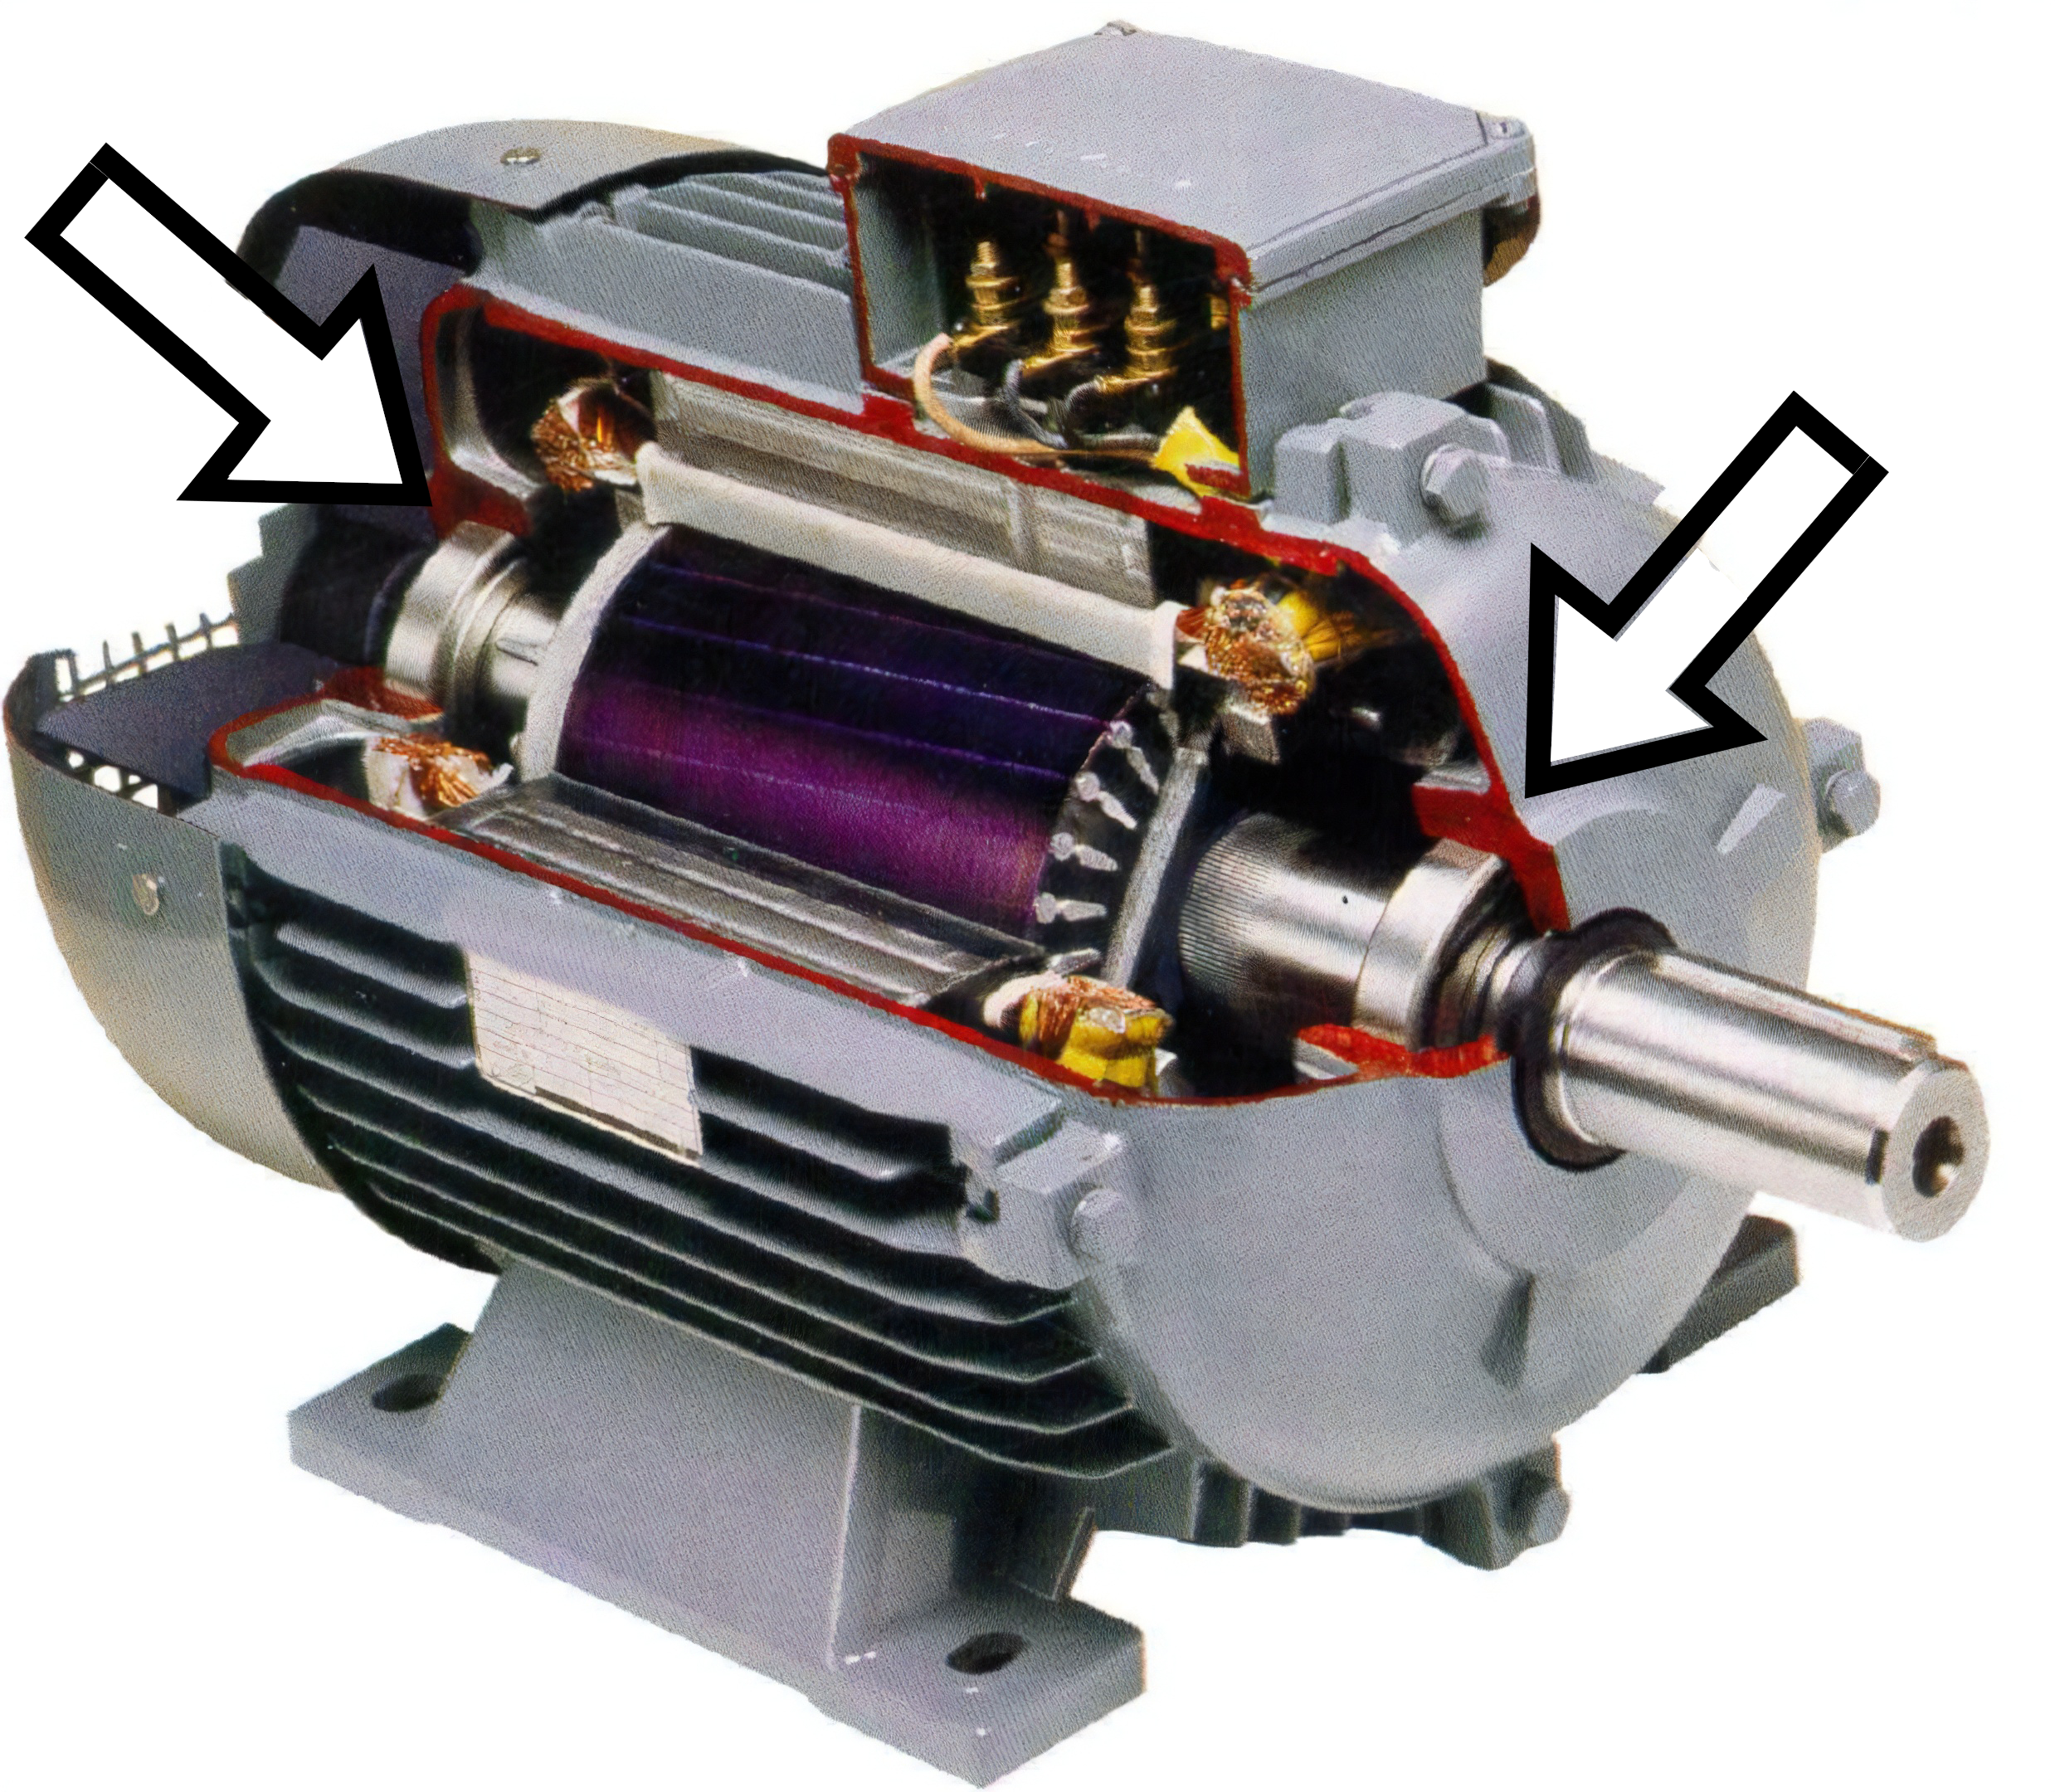
\includegraphics[width=0.7\linewidth]{../images/diapositivas/planteamiento/motor-electrico.png}}
    \only<4>{\includegraphics[width=0.7\linewidth]{../images/diapositivas/planteamiento/rodamiento.jpg}}
    \only<5>{\includegraphics[width=0.9\linewidth]{../images/diapositivas/planteamiento/desgaste-rodamiento.png}}
    \only<6>{\includegraphics[width=0.6\linewidth]{../images/diapositivas/planteamiento/fallas-rodamiento.jpg}}
    \only<7>{\includegraphics[width=0.7\linewidth]{../images/diapositivas/planteamiento/acelerometro.png}}
\end{table}
\end{frame}

\section{Objetivos}

\begin{frame}
   \huge
   Objetivos
\end{frame}

\begin{frame}
    \frametitle{Objetivo General}
    \large
	Desarrollar una herramienta computacional para el análisis de la vibración en
    motores eléctricos, mediante la simulación digital de un acelerómetro, con la
    finalidad de que un operador determine averías y sus causas.
\end{frame}

\begin{frame}
    \frametitle{Objetivos específicos}
    \large
    Justificar la escogencia de las herramientas y lenguajes a utilizar en las diferentes
etapas que requiere la simulación.
\end{frame}

\begin{frame}
    \frametitle{Objetivos específicos}

    \large
    Generar un modelo estadístico de la vibración en motores eléctricos con distinto
nivel de daño utilizando una base de datos de la salida de un acelerómetro
digital.\break \vfill
\pause

    Elaborar una base de datos con información obtenida del modelo estadístico
para alimentar los niveles de análisis de la herramienta.\break
\end{frame}

\begin{frame}
    \frametitle{Objetivos específicos}

    \large
    Realizar análisis de fallas en frecuencia, a partir de la salida del modelo del
acelerómetro.
\end{frame}

\begin{frame}
    \frametitle{Objetivos específicos}

    \large
    Mostrar la información solicitada de acuerdo al nivel de análisis seleccionado.
según sea: Vista Principal, Vista Específica o Vista Exhaustiva.\break\vfill
\pause

    Elaboración de una página Web para facilitar la utilización del sistema\break
\end{frame}

\begin{frame}
    \frametitle{Objetivos específicos}
    \large
    Comprobar los resultados de la herramienta de análisis.\break
\end{frame}

\section{Metodología}

\begin{frame}
   \huge
   Metodología
\end{frame}

%general
\begin{frame}
    \frametitle{Metodología Web}
    \begin{table}
    \only<1>{\includegraphics[width=0.9\linewidth]{../images/diapositivas/metodologia/metodologiaWeb.jpg}}
    \only<2>{\includegraphics[width=0.9\linewidth]{../images/diapositivas/metodologia/metodologiaWeb1.png}}
    \only<3>{\includegraphics[width=0.9\linewidth]{../images/diapositivas/metodologia/metodologiaWeb2.png}}
    \only<4>{\includegraphics[width=0.9\linewidth]{../images/diapositivas/metodologia/metodologiaWeb3.png}}
    \only<5>{\includegraphics[width=0.9\linewidth]{../images/diapositivas/metodologia/metodologiaWeb4.png}}
    \end{table}
\end{frame}

\begin{frame}
    \large
    \frametitle{Metodología Web}
       Fase de desarrollo.\break \pause
        \vfill
        Fase de prueba.
\end{frame}

%Microservicios
%Monolitico
\begin{frame}
    \frametitle{Microservicios}
    \only<1>{\includegraphics[width=\linewidth]{../images/diapositivas/metodologia/microservicioMonolitico.jpg}}
\end{frame}

\begin{frame}
    \frametitle{Microservicios}
    \only<1>{\includegraphics[width=\linewidth]{../images/diapositivas/metodologia/microservicio.jpg}}
\end{frame}

\section{Resultados}
\begin{frame}
   \huge
    Resultados
\end{frame}

\begin{frame}
    \frametitle{Estructura de la aplicación}
    \begin{table}
        \includegraphics[width=0.6\linewidth]{../images/diapositivas/sistema.png}
    \end{table}
\end{frame}

\begin{frame}
    \frametitle{Lenguajes y Herramientas}
    \begin{table}
        \only<1>{\includegraphics[width=\linewidth]{../images/diapositivas/editores.png}}
        \only<2>{\includegraphics[width=0.5\linewidth]{../images/diapositivas/git.jpg}}
        \only<2>{\includegraphics[width=0.5\linewidth]{../images/diapositivas/github.jpg}}
    \end{table}
\end{frame}

\subsection{Análisis exploratorio}
\begin{frame}
    \frametitle{Análisis Exploratorio}
    \begin{table}
        \only<1>{\includegraphics[width=0.6\linewidth]{../images/diapositivas/python.png}}
        \only<2>{\includegraphics[width=\linewidth]{../images/diapositivas/numpy.png}}
        \only<3>{\includegraphics[width=\linewidth]{../images/diapositivas/pandas.jpeg}}
        \only<4>{\includegraphics[width=\linewidth]{../images/diapositivas/scipy.jpg}}
        \only<5>{\includegraphics[width=\linewidth]{../images/diapositivas/matplotlib.png}}
        \only<6>{\includegraphics[width=\linewidth]{../images/diapositivas/modelo/velocidad-horizontal.png}}
        \only<7>{\includegraphics[width=\linewidth]{../images/diapositivas/modelo/velocidad-vertical.png}}
        \only<8>{\includegraphics[width=\linewidth]{../images/diapositivas/modelo/diagrama-dispersion.png}}
        \only<9>{\includegraphics[width=\linewidth]{../images/diapositivas/modelo/diagrama-dispersion-regresion.png}}
        \only<10>{\includegraphics[width=\linewidth]{../images/diapositivas/modelo/magnitud-velocidad.png}}
        \only<11>{\includegraphics[width=\linewidth]{../images/diapositivas/modelo/angulo-velocidad.png}}
        \only<12>{\includegraphics[width=\linewidth]{../images/diapositivas/modelo/aceleracion.png}}
    \end{table}
\end{frame}



\subsection{Base de datos}
\begin{frame}
    \frametitle{Bases de datos}
    \large
    ¿Qué es una Base de datos?\break \pause

    \vfill
    Tipos de Bases de datos.\break
\end{frame}

\begin{frame}
    \frametitle{MongoDB}
    \large
    Clusters\break \pause
    \vfill

    Colecciones y Documentos.\break \pause
    \vfill

    Json $\rightarrow$ Bson.
\end{frame}



\begin{frame}
    \frametitle{Hosting}
    \begin{table}
        \only<1>{\includegraphics[width=\linewidth]{../images/diapositivas/hosting.jpeg}}
        \only<2>{\includegraphics[width=0.6\linewidth]{../images/diapositivas/mongoDB.png}}
    \end{table}
\end{frame}

\begin{frame}
    \frametitle{Colección MotorInDB}
    \begin{table}[ht]
        \begin{center}
            \begin{tabular}{|c|c|p{7cm}|}
                \hline
                Elemento & tipo     & Descripción \\\hline\hline
                %
                \_id      & [ ]bytes  & Elemento utilizado por MongoDB para
                identificar y facilitar la búsqueda de los documentos\\\hline
                %
                IdMotor  & [ ]string & Lista que contiene todos los identificadores
                únicos de los motores. Facilita búsqueda e implementación de los
                clientes Webs\\\hline
            \end{tabular}

            \vspace{0.5cm}
            El símbolo ``[ ]"\ indica que es un arreglo de ese tipo de datos.
        \end{center}
    \end{table}

\end{frame}

\begin{frame}
    \frametitle{Colección MotorData}
    \begin{table}[ht]
        \begin{center}
            \begin{tabular}{|c|c|p{5cm}|}
                \hline
                Elemento        & tipo de dato & Descripción \\\hline\hline
                %
                $\_$id      & [ ]bytes  & Elemento utilizado por MongoDB para
                identificar y facilitar la búsqueda de los documentos\\\hline
                %
                IdMotor         & string   & Identificador único del motor.\\\hline
                %
                Características & string   & Descripción e información del motor.\\\hline
                %
                IdSensor        & [ ]uint64 & lista de los identificadores-sensores
                que tiene conectado este motor.\\\hline
                %
                Data            & [ ]DataSensor & lista en forma de sub colección
                que contiene los resultados del sensor.\\\hline
                %
                Time            & int64  & Estampa de tiempo, fecha y hora de la muestra en formato Unix.\\\hline
            \end{tabular}

            \vspace{0.5cm}
            El símbolo ``[  ]"\  indica que es un arreglo de ese tipo de datos.
        \end{center}
    \end{table}
\end{frame}

\begin{frame}
    \frametitle{Colección MotorData}
    \begin{table}[ht]
        \begin{center}
            \begin{tabular}{|c|c|p{5cm}|}
                \hline
                Elemento        & tipo de dato & Descripción \\\hline\hline
                %
                UmbInferiorVel  & int32  & Umbral Inferior de velocidad.\\\hline
                %
                UmbSuperiorVel  & int32   & Umbral Superior de velocidad.\\\hline
                %
                UmbInferiorAcel & int32   & Umbral Inferior de aceleración.\\\hline
                %
                UmbSuperiorAcel & int32 & Umbral Superior de aceleración.\\\hline
                %
            \end{tabular}
        \end{center}
    \end{table}
\end{frame}

\begin{frame}
    \frametitle{Estructura DataSensor}
    \begin{table}[ht]
        \begin{center}
            \begin{tabular}{|c|c|p{6cm}|}
                \hline
                \multicolumn{3}{|c|}{Sub colección  ``DataSensor"\ }\\\hline\hline
                %
                IdSensorData & uint64 & Identificador único del sensor que tomo la muestra.\\\hline
                Aceleración  & float64 & Muestra de aceleración medida en g .\\\hline
                VelocidadX & float64 & Muestra de velocidad en el eje X.\\\hline
                VelocidadY & float64 & Muestra de velocidad en el eje Y.\\\hline
                VelocidadZ & float64 & Muestra de velocidad en el eje Z.\\
                \hline
            \end{tabular}
        \end{center}
    \end{table}
\end{frame}

\begin{frame}
    \frametitle{Estructura de IdSensor}
    \begin{table}[ht]
        \begin{center}
            \begin{tabular}{|c|c|c|c|}
                \hline
                Tipo de sensor & Reservado& Ubicación   & Serial \\\hline\hline
                $ N_{15} $ & $ N_{14}N_{13} $ &$ N_{12} $  &  $ N_{11}\cdots N_{0} $\\
                \hline
            \end{tabular}

            \vspace{0.3cm}
            \begin{tabular}{|c|p{7cm}|}
                \hline
                Campo       & Descripción
                \\\hline\hline
                tipo        & tipo de sensor usado, Acelerómetro, Temperatura, etc.
                Con $0000b$ siendo Acelerómetro y 15 posibilidades adicionales.
                \\\hline
                Reservado   & No se utilizan, son 0x00 siempre y se reservan para
                posibles expansiones y/o necesidades.
                \\\hline
                Ubicación   & Posición con respecto al motor y acoples. Con:
                $0000b$ Lado con carga, $ 0001b$ Lado libre, $ 0010b\cdots1111b $
                disponibles para acoples y chumaceras.
                \\\hline
                Serial      & número de fabricación del sensor, desde 0 hasta $2^{48}$.
                \\\hline
            \end{tabular}
        \end{center}
    \end{table}
\end{frame}

\subsection{implementación modelo estadísticos}

\begin{frame}
    \frametitle{Modelo estadísticos}
    \begin{table}
        \only<1>{\includegraphics[width=0.9\linewidth]{../images/diapositivas/modelo/prueba-KS.png}}
        \only<2>{\includegraphics[width=0.9\linewidth]{../images/diapositivas/modelo/ajuste-bondad.png}}
        \only<3>{\includegraphics[width=0.6\linewidth]{../images/diapositivas/modelo/rodamiento-golpe.jpg}}
        \only<4>{\includegraphics[width=0.9\linewidth]{../images/diapositivas/modelo/golpeteo.png}}
        \only<5>{\includegraphics[width=0.9\linewidth]{../images/diapositivas/modelo/frecuencia-impacto.png}}
        \only<6>{\includegraphics[width=0.9\linewidth]{../images/diapositivas/modelo/frecuencia-impacto-aventanada.png}}
        \only<7>{\includegraphics[width=0.9\linewidth]{../images/diapositivas/modelo/golpeteo-simulado.png}}
        \only<8>{\includegraphics[width=0.9\linewidth]{../images/diapositivas/modelo/golpeteo-simulado-con-ruido.png}}
    \end{table}
\end{frame}

\begin{frame}
    \frametitle{Hosting}
    \begin{table}
        \includegraphics[width=0.8\linewidth]{../images/diapositivas/digitalOcean.jpeg}
    \end{table}
\end{frame}

\subsection{interconexiones}

\begin{frame}
    \frametitle{API}
    ¿Qué son las API? \break \vfill
    \pause

    ¿Qué ventajas ofrecen?
\end{frame}

\begin{frame}
    \frametitle{FastAPI}
    \begin{table}
        \includegraphics[width=0.9\linewidth]{../images/diapositivas/fastApi.png}
    \end{table}
\end{frame}


\subsection{Microservicio Sensorica}

\begin{frame}
    \frametitle{Golang}
    \begin{table}
    \includegraphics[width=0.9\linewidth]{../images/diapositivas/golangCuchi.jpeg}
    \end{table}
\end{frame}

\begin{frame}
    \frametitle{End Points}
    \begin{table}[H]
        \begin{center}
            \begin{tabular}{|p{4.2cm}|p{5.8cm}|}
                \hline
                Dirección       & Tarea realizada
                \\\hline\hline
                DireccionIP/sensormessage &
                controlar el comportamiento, acceso
                e intercambio de información sensor-servidor.

                Es una comunicación
                bidireccional con Http2 (Https) y se intercambian por el canal
                establecido al comenzar la conexión.
                \\\hline
                DireccionIP/exhaustive \textbf{?idMotor=identificador}   &
                Solicitar la información para la vista exhaustiva,
                el identificador único del motor que se solicita la data
                es enviado por el Url (?idMotor=identificador) .
                \\\hline
            \end{tabular}
        \end{center}
    \end{table}

\end{frame}

\begin{frame}
    \frametitle{Estructura medición exhaustiva}
    \begin{table}[ht]
        \begin{center}
            \begin{tabular}{|c|c|p{5cm}|}
                \hline
                Elemento        & tipo de dato & Descripción \\\hline\hline
                %
                IdMotor         & string   & Identificador único del motor.\\\hline
                %
                Características & string   & Descripción e información del motor.\\\hline
                %
                IdSensor        & [ ]uint64 & lista de los identificadores-sensores
                que tiene conectado este motor.\\\hline
                %
                Data            & [ ]DataExhaustive & lista en forma de sub colección
                que contiene los resultados del sensor.\\\hline
                %
                Time            & int64  & Estampa de tiempo, fecha y hora de la muestra en formato Unix.\\\hline
            \end{tabular}

            \vspace{0.5cm}
            El símbolo ``[  ]"\  indica que es un arreglo de ese tipo de datos.
        \end{center}
    \end{table}
\end{frame}

\begin{frame}
    \frametitle{Estructura DataExhaustiva}
    \begin{table}[ht]
        \begin{center}
            \begin{tabular}{|c|c|p{6cm}|}
                \hline
                \multicolumn{3}{|c|}{estructura  ``DataExhaustiva"\ }\\\hline\hline
                %
                IdSensorData & uint64 & Identificador único del sensor que tomo la muestra.\\\hline
                Data  & []float64 &Lista de mediciones de aceleración, medidas en g.\\\hline
            \end{tabular}

            \vspace{0.5cm}
            El símbolo ``[  ]"\  indica que es un arreglo de ese tipo de datos.
        \end{center}
    \end{table}
\end{frame}


\subsection{Cliente Sensorica}
\begin{frame}
    \frametitle{Cliente Sensorica}
    \begin{table}
    \only<1>{\includegraphics[width=0.65\linewidth]{../images/diapositivas/clients/clienteSensorica.png}}
    \only<2>{\includegraphics[width=0.65\linewidth]{../images/diapositivas/clients/clienteSensorica1.png}}
    \only<3>{\includegraphics[width=0.65\linewidth]{../images/diapositivas/clients/clienteSensorica2.png}}
    \only<4>{\includegraphics[width=0.65\linewidth]{../images/diapositivas/clients/clienteSensorica3.png}}
    \only<5>{\includegraphics[width=0.65\linewidth]{../images/diapositivas/clients/clienteSensorica4.png}}
    \end{table}
\end{frame}





\subsection{Servidor Web}

\begin{frame}
    \frametitle{Servidor Web}
    \begin{table}
        \only<1>{\includegraphics[width=0.9\linewidth]{../images/diapositivas/django.jpg}}
        \only<2>{\includegraphics[width=\linewidth]{../images/diapositivas/djangorest.png}}
    \end{table}
\end{frame}

\begin{frame}
    \frametitle{Servidor Web}
    \begin{table}
        \begin{center}
            \only<1>{
            \begin{tabular}{|p{4.8cm}|p{5.4cm}|}
                \hline
                Dirección       & Tarea realizada
                \\\hline\hline
                DireccionIP/ &
                Enviar los archivos necesarios
                para mostrar la vista general en el navegador.
                \\\hline
                DireccionIP/especifica \textbf{?IdMotor=identificador}&
                Enviar los archivos necesarios
                para mostrar la vista especifica en el navegador.
                \\\hline
                DireccionIP/exhaustiva \textbf{?IdMotor=identificador}  &
                Enviar los archivos necesarios
                para mostrar la vista exhaustiva en el navegador.\\\hline
            \end{tabular}
            }
            \only<2>{
            \begin{tabular}{|p{4.8cm}|p{5.4cm}|}
                \hline
                Dirección       & Tarea realizada
                \\\hline\hline
                DireccionIP/ static/... &
                Envío de
                archivos estáticos por solicitudes externas, ya sea por un
                requerimiento del HTML o del JavaScript.
                \\\hline
                DireccionIP/ get\_data\_motores &
                API que entrega  una lista, formato JSON,
                con la ultima medición almacenada de cada sensor en la base de
                datos.
                \\\hline
                DireccionIP/ get\_list\_motores &
                API que entrega una lista, formato JSON,
                con todos los motores de los que se
                dispone información en la base de datos.\\\hline
            \end{tabular}
            }
            \only<3>{
            \begin{tabular}{|p{4.8cm}|p{5.4cm}|}
                \hline
                Dirección       & Tarea realizada
                \\\hline\hline
                DireccionIP/get\_especifica \textbf{?IdMotor=identificador}&
                API que se encarga de devolver un JSON con toda la información
                en la base de datos referente al motor con el Id pasado en el
                Url, además de las direcciones para las gráficas históricas
                \\\hline
                DireccionIP/get\_exhaustiva \textbf{?IdMotor=identificador}&
                API que se encarga de devolver un JSON con toda la información
                en la base de datos referente al motor con el Id pasado en el
                Url, además de las direcciones para las gráficas históricas
                y exhaustiva.
                \\\hline
                DireccionIP/help&
                Endpoint que se encarga de enviar el HTML referente al manual
                de usuario.\\\hline
            \end{tabular}
            }
        \end{center}
    \end{table}
\end{frame}



\subsection{Cliente Web}
\begin{frame}
    \frametitle{Cliente web}
    \large
    HTML\break \pause
    \vfill
    CSS \break \pause
    \vfill
    JavaScript $\rightarrow$ ReactJs.
\end{frame}


\subsubsection{General}
\begin{frame}
    \frametitle{Cliente Web, vista general}
    \begin{table}
        \begin{center}
    \only<1>{\includegraphics[width=0.6\linewidth]{../images/diapositivas/clients/general.png}}
    \only<2>{\includegraphics[width=0.6\linewidth]{../images/diapositivas/clients/general1.png}}
    \only<3>{\includegraphics[width=0.6\linewidth]{../images/diapositivas/clients/general2.png}}
    \only<4>{\includegraphics[width=0.6\linewidth]{../images/diapositivas/clients/general3.png}}
        \end{center}
    \end{table}
\end{frame}


\subsubsection{Específica}
\begin{frame}
    \begin{table}
    \frametitle{Cliente Web, vista específica}
    \only<1>{\includegraphics[width=0.9\linewidth]{../images/diapositivas/clients/es1.png}}
    \end{table}
\end{frame}

\begin{frame}
    \frametitle{Cliente Web, vista específica}
     \begin{table}[H]
        \begin{center}
            \begin{tabular}{p{5cm}p{5cm}}

            \includegraphics[width=5cm]{../images/diapositivas/clients/as_medio2.png}&
            \includegraphics[width=5cm]{../images/diapositivas/clients/vxs_medio2.png}\\
            \includegraphics[width=5cm]{../images/diapositivas/clients/vys_medio2.png}&
            \includegraphics[width=5cm]{../images/diapositivas/clients/vzs_medio2.png}\\

            \end{tabular}
        \end{center}
    \end{table}
\end{frame}

\begin{frame}
    \begin{table}
    \frametitle{Cliente Web, vista específica}
    \includegraphics[width=0.7\linewidth]{../images/diapositivas/clients/tabla.jpg}
    \end{table}
\end{frame}


\subsubsection{Exhaustiva}
\begin{frame}
    \frametitle{Cliente Web, vista exhaustiva}
    \begin{table}
    \only<1>{\includegraphics[width=0.5\linewidth]{../images/diapositivas/clients/ex1.png}}
    \only<2>{\includegraphics[width=0.5\linewidth]{../images/diapositivas/clients/ex3.png}}
    \only<3>{\includegraphics[width=0.5\linewidth]{../images/diapositivas/clients/ex2.png}}
    \only<4>{\includegraphics[width=0.5\linewidth]{../images/diapositivas/clients/es4.png}}
    \end{table}
\end{frame}

\subsection{Scripts}
\begin{frame}
    \frametitle{Scripts}
    \large
    ¿Qué son?\\ \pause
    \vfill
    ¿En que lenguajes se pueden implementar?
\end{frame}

\begin{frame}
    \frametitle{Llenado de la base de datos}
    \begin{table}
        \includegraphics[width=0.9\linewidth]{../images/diapositivas/scriptLlenarBBDD.png}
    \end{table}
\end{frame}

\begin{frame}
    \frametitle{Sensor}
    \begin{table}
        \includegraphics[width=0.9\linewidth]{../images/diapositivas/scriptSensor.jpg}
    \end{table}
\end{frame}


\subsection{Comprobación de resultados}

\begin{frame}
    \huge
    Comprobación de resultados
\end{frame}

\begin{frame}
    \frametitle{Comprobación tecnica}
    \begin{table}
        \only<1>{\includegraphics[width=\linewidth]{../images/comprobacion_resultados/tecnicos/reinicio_servidor.png}}
        \only<2>{
            \includegraphics[width=0.6\linewidth]{../images/diapositivas/noUnicidad1.png} \break
            \includegraphics[width=0.6\linewidth]{../images/diapositivas/noUnicidad2.png}
        }
        \only<3>{\includegraphics[width=\linewidth]{../images/comprobacion_resultados/tecnicos/conexionInvalidaNoBBDDSensorica.png}}
        \only<4>{\includegraphics[width=\linewidth]{../images/comprobacion_resultados/tecnicos/conexionInvalidaNoBBDDWeb.png}}
        \only<5>{\includegraphics[width=\linewidth]{../images/comprobacion_resultados/tecnicos/conexionInvalidaNoMotorSensorica.png}}
        \only<6>{\includegraphics[width=\linewidth]{../images/comprobacion_resultados/tecnicos/redireccionClienteWeb.png}}
    \end{table}
\end{frame}

\begin{frame}
    \frametitle{Comprobación de resultados}
    \begin{table}
        \only<1-3>{
            \begin{tabular}{m{6cm}m{6cm}}
            \only<1>{
                \includegraphics[width=6cm]{../images/comprobacion_resultados/finales/n1.png}&
                \includegraphics[width=6cm]{../images/comprobacion_resultados/finales/n1mongo.png}\\
            }
            \only<2>{
                \includegraphics[width=6cm]{../images/comprobacion_resultados/finales/n2.png}&
                \includegraphics[width=6cm]{../images/comprobacion_resultados/finales/n2mongo.png}\\
            }
            \only<3>{
                \includegraphics[width=6cm]{../images/comprobacion_resultados/finales/n3.png}&
                \includegraphics[width=6cm]{../images/comprobacion_resultados/finales/n3mongo.png}
            }
            \end{tabular}
            }
        \only<4-5>{
            \begin{tabular}{m{6cm}m{6cm}}
            \only<4>{
                \includegraphics[width=6cm]{../images/comprobacion_resultados/finales/f1.png}&
                \includegraphics[width=6cm]{../images/comprobacion_resultados/finales/f1mongo.png}\\
            }
            \only<5>{
                \includegraphics[width=6cm]{../images/comprobacion_resultados/finales/f2.png}&
                \includegraphics[width=6cm]{../images/comprobacion_resultados/finales/f2mongo.png}
            }
            \end{tabular}
        }
        \only<6>{ \includegraphics[width=7cm]{../images/diapositivas/com1.png}        }
        \only<7>{ \includegraphics[width=7cm]{../images/diapositivas/com2.png}        }
        \only<8>{
            \includegraphics[width=10cm]{../images/comprobacion_resultados/finales/comFFT2.png}
        }
    \end{table}
\end{frame}

\section{Conclusiones}
\begin{frame}
    \frametitle{Conclusiones}
     El desarrollo  de una herramienta computacional para el análisis de
    la vibración en motores eléctricos se hizo posible mediante la
    implementación de dos servidores, uno de estilo
    microservicio y un cliente Web, puede ser alimentada mediante la
    simulación de un  modelo estadístico o
    mediante mediciones a tiempo real de cualquier sistema
    que respete las estructuras de datos empleado.
\end{frame}

\begin{frame}
    \frametitle{Conclusiones}
    Se implementaron múltiples servicios, cada uno escrito con un
    lenguaje de programación que satisface los requerimientos de velocidad,
    paralelismo y robustez necesarios para  los requerimientos de
    uso, además de una fácil adecuación y modificación a las necesidades,
    de múltiples clientes.
\end{frame}

\begin{frame}
    \frametitle{Conclusiones}
    Existe una gran cantidad de lenguajes de programación en la actualidad
    diseñados para satisfacer una gran cantidad de tareas en múltiples campos,
    siendo Go y Python herramientas de gran poder y fácil implementación
    al realizar servidores y API, además de la creación de Script
    para la automatización de procesos; de igual forma Python es increíblemente
    polifacético y cuenta con una gran cantidad de librerías y Frameworks
    especialmente en el área de la ciencia de datos y estadística.
\end{frame}

\begin{frame}
    \frametitle{Conclusiones}
     En términos de programación Web a nivel cliente,
    HTML, CSS, JavaScript, son casi una obligación, sin embargo,
    JavaScript cuenta con una  variedad de Frameworks para agilizar el
    trabajo, siendo React uno
    de los mas utilizados en la industria.
\end{frame}


\begin{frame}
    \frametitle{Conclusiones}
     Se implementaron dos modelos estadísticos, uno para entregar el
    equivalente a mediciones diarias y otro para mediciones continuas a tiempo
    real necesarias para hacer un análisis en frecuencia,
    utilizando distribuciones de probabilidad para representar 3 variables de interés,
    velocidad vertical, horizontal y aceleración, expresadas de forma independiente
    como magnitud y ángulo de la velocidad y aceleración las dos primeras
    siendo representadas en coordenadas polares.
\end{frame}

\begin{frame}
    \frametitle{Conclusiones}
            Las distribuciones que satisfacen de mejor manera las variables
        modeladas fueron la distribución Burr
        de tipo III, para la magnitud de velocidad y aceleración, y la distribución
        normal para el ángulo, de esta forma se obtienen las mediciones diarias;
        con un modelo de señal no estadístico ajustado a la amplitud, dada por
        el modelo de la aceleración, mas una gaussiana, para simular ruido, se obtienen
        las mediciones continuas.
\end{frame}


\begin{frame}
    \frametitle{Conclusiones}
        Se implementó una API Web, para facilitar la accesibilidad al modelo, con
        el Frameworks FastAPI y dos endpoints que entregan la información especificada
        en el Url y en los parámetros de configuración, nivel de daño (un número del 0 al 10)
        y el identificador único del motor que tiene asociado.
\end{frame}

\begin{frame}
    \frametitle{Conclusiones}
    El análisis en frecuencia se realiza mediante una
        transformada rápida de Fourier (FFT) lo que permite llevar la señal
        discretizada (mediciones a tiempo real) al dominio de la frecuencia
        y posteriormente graficarla; todo esto se logra mediante las librerías
        \textbf{numpy} y \textbf{matplotlib} de Python.
\end{frame}

\begin{frame}
    \frametitle{Conclusiones}
        Se utilizó una base de datos no relacional, \textbf{MongoDB}, en forma
        de microservicio con la empresa \textbf{MongoDB Atlas};
        esta base de datos llamada \textbf{tesis}
        contiene 2 colecciones, una se encarga de almacenar la información de las
        mediciones diarias y la otra de almacenar los identificadores únicos que
        representan a los motores de los que se posee información.
\end{frame}


\begin{frame}
    \frametitle{Conclusiones}
        La automatización de procesos es fundamental para agilizar las tareas y
        la forma mas sencilla y eficiente de hacerlo fue mediante un Script.
\end{frame}

\begin{frame}
    \frametitle{Conclusiones}
    \large
        Se crearon 2 microservicios:
        \begin{itemize}
            \item{servidor de sensorica}
            \item{servidor Web},
        \end{itemize}
\end{frame}

\begin{frame}
    \frametitle{Conclusiones}
    \large
        Facilitar la utilización del modelo estadístico y la conexión con
        el microservicio de \textbf{sensorica} se implementó con un \textbf{cliente de
        sensorica} escrito en Go el cual permitió especificar las características
        inherentes al motor (Identificador del motor y de los sensores, características, etc)
        y al daño existente en el mismo (en una escala del 1 al 10), además,
        especificar la dirección IP, o puerto local, al cual se conectará.
\end{frame}

\begin{frame}
    \frametitle{Conclusiones}
    \large
        Se crearon 3 vistas para el cliente Web, estas son:
        \begin{itemize}
            \item \textbf{General}, con el cual se conoce el estado de todos
                los motores registrados en la base de datos, mediante paginación
                en una ventana se muestran 12 motores por vez, y controlar
                cuáles son mostrados,
                y especificar el identificador
                único del motor del cual se quiere obtener mas información.
                %
            \item \textbf{Específica},
                muestra la evolución histórica del motor mediante gráficas
                y una tabla exportable a Excel; adicionalmente permite solicitar
                la vista exhaustiva.
                %
            \item \textbf{Exhaustiva},
                solicita mediciones a tiempo real de la aceleración del motor
                y las descompone en frecuencia, permitiendo observar una gráfica
                de las frecuencias y magnitudes  en las que vibra
                el motor; adicionalmente muestra toda la información de la
                vista específica.
        \end{itemize}

\end{frame}

\begin{frame}
    \frametitle{Conclusiones}
    \large
        Se probó manualmente el sistema en los puntos claves
        e interconexiones, con lo cual  se comprobó:
        \begin{itemize}
            \item La unicidad de la información.
            \item Fallas de conexión con el microservicio de base de datos.
            \item Solicitud de información a tiempo real a un motor sin conexión
                establecida.
            \item Peticiones invalidas en el servidor Web
        \end{itemize}
\end{frame}

\begin{frame}
    \frametitle{Conclusiones}
    \large
        Se comprobó el cumplimiento de
        los requerimientos mínimos que satisfacen las condiciones planteadas,
        mediante la
        demostración de la clasificación en los distintos niveles de daño,
         se corroboró la coherencia y legibilidad
        de las gráficas históricas y de la gráfica del análisis en frecuencia.
\end{frame}


\section{Recomendaciones}

\begin{frame}
    \frametitle{Recomendaciones}
    Utilizar un sistema de adquisición de datos, sensores o placas diseñadas
    para la obtención de las mediciones diarias, por ejemplo los datos a tiempo
    real para alimentar el sistema.

\end{frame}

\begin{frame}
    \frametitle{Recomendaciones}
        Implementar un sistema de autenticación y seguridad para que solo
    los usuarios con los
    privilegios correctos puedan acceder a la información, esto
    probablemente requiera el uso de otra base de datos preferiblemente
    relacional, y de esta forma poder hacer uso empresarial
    de la aplicación.
\end{frame}

\begin{frame}
    \frametitle{Recomendaciones}
    Un sistema de notificaciones configurable por el usuario,
    puede ser una gran ayuda al operador de la aplicación en el diagnóstico
    de fallas de forma temprana, para observar si algún motor recibe una
    medida fuera de los valores normales.
\end{frame}

\begin{frame}
    \frametitle{Recomendaciones}
    Debido a la complejidad de las conexiones HTTP2 una alternativa es el
    uso de Websockets los cuales permiten una conexión bidireccional sin la
    complejidad del nuevo protocolo evaluando  los requerimientos
    de la aplicación. Otra alternativa, en un futuro
    cercano, posiblemente lo sea el HTTP3 la cual está siendo discutida
    por el comité del estándar HTTP para corregir fallas de la última
    versión.
\end{frame}

\begin{frame}
    \frametitle{Recomendaciones}
    Creación y uso de  pruebas automatizadas para minimizar el tiempo de
    depuración y evitar fallas en producción, cabe destacar que esto
    implica un coste
    en el tiempo de desarrollo dedicado al diseño de las pruebas.
    La elección de usarlas dependerá de la experiencia previa
    del programador con este tipo de metodología de desarrollo.
\end{frame}

\end{document}

